\documentclass[12pt]{article}
\usepackage[a4paper, margin=2.5cm]{geometry}
\usepackage[utf8]{inputenc}
\usepackage[T1]{fontenc}
\usepackage{setspace}
\onehalfspacing
\usepackage{graphicx}
\usepackage{amsmath, amssymb}
\usepackage{booktabs}
\usepackage{caption}
\usepackage{float}
\usepackage{hyperref}

\title{Econometrics II -- Assignment 4:\\
Volatility Timing in the U.S. Stock Market}
\date{Spring 2026}

\begin{document}

\maketitle
% ─────────────────────────────────────────────────────────────────────────────
\section{Introduction}
% ─────────────────────────────────────────────────────────────────────────────

This report asks two linked questions about monthly U.S.\ stock-market log excess returns, $x_t=\text{mkt}_t-\text{rf}_t$, from July 1926 to February 2026. First, do excess returns exhibit ARCH effects and asymmetric (leverage) volatility responses? Second, can a conditional-variance forecast from such a model be used to construct a volatility-targeted portfolio that outperforms both the unscaled market and the expanding-window benchmark in (2.1) of the assignment?

The motivation is the evidence in Harvey et al.\ (2018) and Moreira and Muir (2017) that volatility targeting improves Sharpe ratios because conditional expected returns do not move one-for-one with conditional volatility. We model the conditional variance with a GJR-GARCH(1,1) under Student-$t$ innovations, estimated by quasi-maximum likelihood. ARCH effects are highly significant, the asymmetry parameter is significantly positive (negative shocks raise next-period variance more than positive shocks of equal size), and the resulting volatility-scaled return $x^*_t$ delivers an annualized Sharpe ratio of $0.43$ versus $0.34$ for the unscaled series and $0.35$ for the expanding-window benchmark. A spanning regression with HAC standard errors confirms that $x^*_t$ generates a positive and statistically significant alpha relative to $x_t$, whereas the expanding-window benchmark does not.

% ─────────────────────────────────────────────────────────────────────────────
\section{Description of the Data}
% ─────────────────────────────────────────────────────────────────────────────

The data are monthly, in percent per month, from Kenneth French's Data Library: $\text{mkt}_t$ is the log return on the value-weighted CRSP market portfolio and $\text{rf}_t$ is the log one-month T-bill rate, both transformed from the published simple returns as continuously compounded equivalents. The sample contains $T=1{,}196$ observations, 1926M7--2026M2. We work throughout with the log excess return $x_t=\text{mkt}_t-\text{rf}_t$.

Figure~\ref{fig:panel} shows that $x_t$ has near-zero serial correlation but $|x_t|$ and $x_t^2$ display strong and slowly decaying autocorrelation: the classic volatility-clustering pattern. Large clusters coincide with 1929--32, 1987, 2008 and 2020. Table~\ref{tab:desc} summarizes the moments: $x_t$ has a positive mean of $0.55\%$ per month, a standard deviation of $5.30\%$, negative skewness ($-0.52$) and pronounced excess kurtosis ($6.48$), which already signals fat tails relative to a Gaussian.

\begin{figure}[H]
\centering

\includegraphics[width=0.95\textwidth]{figures/fig1_series_panel.pdf}
\caption{Top: $x_t$ and $|x_t|$. Bottom: sample ACFs of $x_t$ and $x_t^2$. The flat ACF of $x_t$ and the persistent ACF of $x_t^2$ motivate a constant-mean ARCH-type model.}
\label{fig:panel}
\end{figure}

% ─────────────────────────────────────────────────────────────────────────────
\section{Econometric Theory}
% ─────────────────────────────────────────────────────────────────────────────

\paragraph{Model.} Given the absence of autocorrelation in $x_t$, we use a constant-mean specification
\begin{equation}
x_t=\mu+\varepsilon_t,\qquad \varepsilon_t=\sigma_t z_t,\qquad z_t\sim \text{iid}(0,1),
\label{eq:mean}
\end{equation}
where $\sigma_t^2=\mathbb{V}[x_t\mid\mathcal{I}_{t-1}]$ depends on past information. We compare nested specifications for $\sigma_t^2$:
\begin{align}
\text{ARCH}(q):\quad &\sigma_t^2=\omega+\textstyle\sum_{j=1}^q\alpha_j\varepsilon_{t-j}^2,
   \label{eq:arch}\\
\text{GARCH}(1,1):\quad &\sigma_t^2=\omega+\alpha\varepsilon_{t-1}^2+\beta\sigma_{t-1}^2,
   \label{eq:garch}\\
\text{GJR-GARCH}(1,1):\quad &\sigma_t^2=\omega+\alpha\varepsilon_{t-1}^2+\kappa\,\varepsilon_{t-1}^2\,\mathbb{I}(\varepsilon_{t-1}<0)+\beta\sigma_{t-1}^2.
   \label{eq:gjr}
\end{align}
For positive variances we require $\omega>0$ and the slope parameters non-negative. Covariance stationarity requires $\sum_j\alpha_j<1$ in (\ref{eq:arch}), $\alpha+\beta<1$ in (\ref{eq:garch}) and, with $\mathbb{E}[\mathbb{I}(\varepsilon_{t-1}<0)]=1/2$ under a symmetric distribution, $\alpha+\beta+\tfrac12\kappa<1$ in (\ref{eq:gjr}). The unconditional variance for GARCH(1,1) is $\sigma^2=\omega/(1-\alpha-\beta)$. In (\ref{eq:gjr}) a positive $\kappa$ encodes the \emph{leverage effect}: negative shocks raise next-period variance by $(\alpha+\kappa)\varepsilon_{t-1}^2$ versus $\alpha\varepsilon_{t-1}^2$ for positive shocks.

\paragraph{Estimator.} Stacking the parameter vector $\theta$, we estimate by (quasi-)maximum likelihood, maximising the Gaussian log-likelihood
\begin{equation}
\ell_T(\theta)=-\tfrac12\sum_{t=1}^{T}\Big[\log(2\pi)+\log\sigma_t^2(\theta)+\frac{(x_t-\mu)^2}{\sigma_t^2(\theta)}\Big].
\label{eq:loglik}
\end{equation}
When $z_t$ is non-Gaussian the Gaussian likelihood is mis-specified but the MLE remains a QMLE: under regularity (correct conditional-variance specification, stationarity, finite fourth moments of $\varepsilon_t$, and an identification condition on $\theta_0$) it is consistent and asymptotically normal,
\[
\sqrt{T}(\hat\theta-\theta_0)\xrightarrow{d}\mathcal{N}\big(0,\mathcal{I}^{-1}\mathcal{J}\,\mathcal{I}^{-1}\big),
\]
with $\mathcal{I}$ the expected Hessian and $\mathcal{J}$ the expected outer product of scores; under Gaussian $z_t$, $\mathcal{J}=\mathcal{I}$ and the variance simplifies to $\mathcal{I}^{-1}$. We report the sandwich SEs. Following the course we also estimate the model with $z_t\sim t(\nu)/\sqrt{\nu/(\nu-2)}$ (scaled Student-$t$); this delivers fully efficient ML inference when innovations are leptokurtic.

\paragraph{Hypotheses and tests.} For the existence of ARCH effects we use the Engle/Breusch--Pagan LM test on $\hat\varepsilon_t$ from a mean-only regression: under $H_0$ of conditional homoskedasticity in (\ref{eq:arch}), $\zeta_{\text{ARCH}}=TR^2\xrightarrow{d}\chi^2(h)$ for the auxiliary regression of $\hat\varepsilon_t^2$ on $h$ of its own lags. Asymmetry is tested with $H_0:\kappa=0$ in (\ref{eq:gjr}) via a robust $t$-test, and by likelihood ratio against GARCH(1,1). Standardized residuals $\hat z_t=\hat\varepsilon_t/\hat\sigma_t$ from the fitted model are inspected with (i) Ljung--Box on $\hat z_t$ and $\hat z_t^2$ (null: no autocorrelation; $\xi_{LB}\sim\chi^2(h)$), (ii) a repeat ARCH-LM test on $\hat z_t$ and (iii) the Jarque--Bera normality test. Finally, the spanning regression
\begin{equation}
x^*_t=\alpha+\beta x_t+u_t \label{eq:span}
\end{equation}
is estimated by OLS with Newey--West HAC SEs at $\lfloor 4(T/100)^{2/9}\rfloor=6$ lags; a positive, significant $\hat\alpha$ indicates that volatility timing improves the unconditional Sharpe ratio.

% ─────────────────────────────────────────────────────────────────────────────
\section{Empirical Analysis}
% ─────────────────────────────────────────────────────────────────────────────

\paragraph{Preliminary tests.} The ARCH-LM test in Table~\ref{tab:archlm} rejects $H_0$ massively at $h\in\{1,5,12\}$ with $p<10^{-15}$: ARCH effects in $x_t$ are unambiguous.

\paragraph{Model selection (general-to-specific).} Table~\ref{tab:models} reports five candidate specifications, all with a constant mean. We start with ARCH($q$) and increase $q$: ARCH(1) fails the LB$(\hat z^2)$ and residual ARCH tests, ARCH(5) absorbs most clustering but still has heavy parameters and relatively poor information criteria. GARCH(1,1) is a strict improvement on both AIC ($7063.4$ vs.\ $7134.7$) and BIC and yields standardized-residual diagnostics that comfortably accept the null of no remaining ARCH structure (LB$(\hat z^2,12)$ $p=0.97$, ARCH$(12)$ $p=0.97$). Persistence $\hat\alpha+\hat\beta=0.98$ is high but well below unity. Adding the asymmetry term gives GJR-GARCH(1,1) with $\hat\kappa=0.125$ ($\hat\sigma_{\hat\kappa}=0.070$, $t=1.79$) and an LR statistic of $2(3527.7-3521.7)=12.0\sim\chi^2(1)$, $p<0.001$; AIC and BIC fall further. Replacing Gaussian innovations by Student-$t(\nu)$ delivers a large jump in fit ($\Delta\log L=34.3$, $\Delta\text{AIC}=-66.6$), an estimated $\hat\nu\approx 7.1$ with $\hat\sigma_{\hat\nu}=1.55$ (decisively rejecting Gaussianity), and a sharper, more significant asymmetry estimate ($\hat\kappa=0.179$, $t=2.93$, $p=0.003$). We therefore select GJR-GARCH(1,1)-$t$ as our preferred model.

\paragraph{Misspecification of the preferred model.} For GJR-$t$ the standardized residuals show no autocorrelation (LB$_{12}$ $p=0.32$), no residual ARCH (LB$(\hat z^2,12)$ $p=0.95$, ARCH$(12)$ $p=0.94$), and the implied persistence $\hat\alpha+\hat\beta+\tfrac12\hat\kappa=0.922$ satisfies covariance-stationarity. Jarque--Bera still rejects normality of $\hat z_t$ ($p<0.001$); this is expected and is exactly the leptokurtosis the $t$ distribution accounts for, so QMLE-with-sandwich inference (and the parametric $t$ likelihood) remain valid. Diagnostics are reported \emph{before} statistical interpretation, in accordance with the course's general-to-specific protocol.

\paragraph{Interpretation.} The preferred estimates (Table~\ref{tab:pref}) say $\hat\mu=0.86$ percent per month (highly significant), and a volatility process dominated by smoothing ($\hat\beta=0.80$) with a small symmetric ARCH effect ($\hat\alpha=0.03$, not individually significant) and a sizable leverage component ($\hat\kappa=0.18$). Economically: a $-5\%$ shock raises next-period $\sigma_t^2$ roughly $(\hat\alpha+\hat\kappa)/\hat\alpha\approx 7$ times more than a $+5\%$ shock, in line with the leverage/volatility-feedback narrative.

\paragraph{Volatility-targeting performance.} Using $\hat\sigma_t$ from the preferred model we form $x^*_t=(\bar\sigma/\hat\sigma_t)x_t$ with $\bar\sigma=10/\sqrt{12}\approx 2.89$ (percent). Figure~\ref{fig:sigma} contrasts $\hat\sigma_t$ with the expanding-window benchmark $\hat\sigma^{ew}_t$: the GJR-$t$ estimate reacts much more sharply to clustering episodes, especially the asymmetric down-moves. Table~\ref{tab:perf} reports performance over the common sample (1928M7--2026M2, $T=1{,}172$). The annualized Sharpe ratio rises from $0.34$ for $x_t$ to $0.43$ for $x^*_t$, while the expanding-window benchmark gives only $0.35$. Excess kurtosis and the worst-month drawdown also improve substantially for $x^*_t$ ($-19.6\%$ vs.\ $-33.9\%$ for $x_t$). Figure~\ref{fig:cum} shows that $x^*_t$ produces a higher and smoother cumulative log return than $x_t$ over the full sample. Table~\ref{tab:span} formalises the comparison via the spanning regression (\ref{eq:span}): for $x^*_t$ the HAC-robust intercept is $\hat\alpha=0.095$ ($t=2.50$, $p=0.013$), so we reject $H_0:\alpha=0$ and conclude that the GJR-$t$ scaling adds genuine risk-adjusted value beyond the unscaled market. For the expanding-window benchmark $\hat\alpha=0.011$ with $t=0.59$ ($p=0.56$): we cannot reject zero alpha, consistent with that benchmark being too slow-moving relative to actual conditional volatility.

% ─────────────────────────────────────────────────────────────────────────────
\section{Discussion}
% ─────────────────────────────────────────────────────────────────────────────

Several caveats apply. (i) The conditional standard deviation $\hat\sigma_t$ used to construct $x^*_t$ is extracted from a model estimated on the full sample, so the strategy is not strictly tradeable in real time; this is the same in-sample evaluation used in the assignment appendix. A genuine out-of-sample exercise would re-estimate $\hat\theta$ on an expanding window and use one-step-ahead variance forecasts, $\hat\sigma_{t|t-1}^2=\hat\omega+(\hat\alpha+\hat\kappa\mathbb{I}_{\varepsilon_{t-1}<0})\varepsilon_{t-1}^2+\hat\beta\hat\sigma_{t-1}^2$. (ii) Inference is conditional on the GJR-$t$ being correctly specified; if the conditional-mean model is too parsimonious (e.g.\ a small but real risk-premium component proportional to $\sigma_t$) some explanatory power would be miscoded as volatility. (iii) The spanning test is unconditional and does not adjust for transaction costs, financing costs, or leverage constraints required to deliver the targeted $10\%$ annualized volatility in low-$\hat\sigma_t$ months. (iv) Jarque--Bera still rejects on $\hat z_t$, indicating residual non-normality beyond what $t(7.1)$ captures; this primarily affects extreme-tail probabilities, not the consistency of the QMLE point estimates.

% ─────────────────────────────────────────────────────────────────────────────
\section{Conclusion}
% ─────────────────────────────────────────────────────────────────────────────

U.S.\ monthly excess returns exhibit strong ARCH effects and statistically significant asymmetric volatility responses. A GJR-GARCH(1,1) with Student-$t$ innovations passes all standard misspecification tests and is the preferred model in our general-to-specific search. Scaling realised returns by its conditional standard deviation raises the annualized Sharpe ratio from $0.34$ to $0.43$ and produces a positive, HAC-significant alpha against the unscaled market, whereas the expanding-window benchmark in (2.1) of the assignment does not. The evidence supports the volatility-timing thesis of Moreira and Muir (2017) and Harvey et al.\ (2018), conditional on the in-sample caveats above.

% ─────────────────────────────────────────────────────────────────────────────
\clearpage
\appendix
\setlength{\abovecaptionskip}{1pt}
\setlength{\belowcaptionskip}{1pt}
\setlength{\textfloatsep}{4pt}
\setlength{\intextsep}{4pt}
\renewcommand{\arraystretch}{0.88}
\scriptsize

\noindent
\begin{minipage}[t]{0.46\linewidth}\centering
\captionof{table}{Descriptive stats, 1926M7--2026M2.}\label{tab:desc}
\begin{tabular}{lrrrrrr}\toprule
Series & Mean & Std & Min & Max & Skew & Ex. Kurt \\\midrule
$\text{mkt}_t$ & 0.817 & 5.289 & -33.84 & 32.87 & -0.55 & 6.53 \\
$\text{rf}_t$ & 0.269 & 0.248 & -0.06 & 1.34 & 1.09 & 1.40 \\
$x_t$ & 0.548 & 5.297 & -33.87 & 32.77 & -0.52 & 6.48 \\
\bottomrule\end{tabular}

\end{minipage}\hfill
\begin{minipage}[t]{0.26\linewidth}\centering
\captionof{table}{ARCH-LM, $H_0$: no ARCH.}\label{tab:archlm}
\begin{tabular}{lcc}\toprule
Lags $h$ & $\zeta_{\mathrm{ARCH}}=T R^2$ & $p$-value \\\midrule
1 & 65.27 & 6.53e-16 \\
5 & 134.43 & 2.73e-27 \\
12 & 236.71 & 8.04e-44 \\
\bottomrule\end{tabular}

\end{minipage}\hfill
\begin{minipage}[t]{0.24\linewidth}\centering
\captionof{table}{Preferred (GJR-$t$).}\label{tab:pref}
\begin{tabular}{lrr}\toprule
Parameter & Estimate & Robust SE \\\midrule
$\mu$ & 0.8582 & 0.1229 \\
$\omega$ & 1.5672 & 0.5535 \\
$\alpha$ & 0.0298 & 0.0216 \\
$\kappa$ & 0.1787 & 0.0609 \\
$\beta$ & 0.8033 & 0.0461 \\
$\nu$ & 7.1011 & 1.5476 \\
\midrule
Persistence $\alpha+\beta+\tfrac12\kappa$ & 0.9224 & \\
$\log L$ & -3487.43 & \\
$T$ & 1196 & \\
\bottomrule\end{tabular}

\end{minipage}

\vspace{0.6em}
\begin{table}[H]\centering
\caption{Model comparison. Robust (sandwich) SEs in parentheses; (Q)MLE with constant mean. Persistence is $\sum_j\alpha_j$ for ARCH($q$), $\alpha+\beta$ for GARCH(1,1), $\alpha+\beta+\tfrac12\kappa$ for GJR. $p$-values: Ljung--Box at $h{=}12$ on $\hat z_t$ and $\hat z_t^2$, ARCH-LM at $h{=}12$ on $\hat z_t$, Jarque--Bera on $\hat z_t$.}\label{tab:models}
\begin{tabular}{lccccc}\toprule
Parameter & ARCH(1) & ARCH(5) & GARCH(1,1) & GJR(1,1) & GJR(1,1)-t \\\midrule
$\mu$ & 0.732 & 0.694 & 0.716 & 0.639 & 0.858 \\
 & (0.157) & (0.145) & (0.125) & (0.120) & (0.123) \\
$\omega$ & 21.966 & 10.498 & 0.734 & 1.029 & 1.567 \\
 & (2.610) & (2.521) & (0.292) & (0.516) & (0.554) \\
$\alpha$ & 0.205 & 0.653 & 0.135 & 0.055 & 0.030 \\
 &  &  & (0.026) & (0.035) & (0.022) \\
$\kappa$ (asym.) & -- & -- & -- & 0.125 & 0.179 \\
 &  &  &  & (0.070) & (0.061) \\
$\beta$ & -- & -- & 0.845 & 0.840 & 0.803 \\
 &  &  & (0.028) & (0.039) & (0.046) \\
$\nu$ & -- & -- & -- & -- & 7.10 \\
 &  &  &  &  & (1.548) \\
\midrule
Persistence & 0.205 & 0.653 & 0.980 & 0.957 & 0.922 \\
$\log L$ & -3646.8 & -3560.4 & -3527.7 & -3521.7 & -3487.4 \\
AIC & 7299.6 & 7134.7 & 7063.4 & 7053.5 & 6986.9 \\
BIC & 7314.8 & 7170.3 & 7083.7 & 7078.9 & 7017.4 \\
\midrule
LB$(\hat z,12)$ $p$ & 0.085 & 0.345 & 0.299 & 0.252 & 0.320 \\
LB$(\hat z^2,12)$ $p$ & $<$0.001 & 0.490 & 0.968 & 0.946 & 0.949 \\
ARCH$(12)$ $p$ & $<$0.001 & 0.459 & 0.969 & 0.944 & 0.944 \\
JB $p$ & $<$0.001 & $<$0.001 & $<$0.001 & $<$0.001 & $<$0.001 \\
\bottomrule\end{tabular}

\end{table}

\vspace{0.4em}\noindent
\begin{minipage}[t]{0.62\linewidth}\centering
\captionof{table}{Performance over common sample (1928M7--2026M2, $T{=}1{,}172$). Sharpe annualized; returns in \% per month.}\label{tab:perf}
\begin{tabular}{lrrrrrrr}\toprule
Series & Mean & Std & Sharpe (ann.) & Skew & Ex.\ Kurt & Min & Max \\\midrule
$x_t$ (unscaled) & 0.525 & 5.327 & 0.342 & -0.52 & 6.45 & -33.87 & 32.77 \\
$x^*_t$ (GJR-$t$) & 0.360 & 2.915 & 0.428 & -0.97 & 3.36 & -19.56 & 8.87 \\
$\text{xs\_scaled\_bt}$ & 0.238 & 2.376 & 0.347 & -0.90 & 5.08 & -15.74 & 9.74 \\
\bottomrule\end{tabular}

\end{minipage}\hfill
\begin{minipage}[t]{0.36\linewidth}\centering
\captionof{table}{Spanning regression (\ref{eq:span}); OLS with Newey--West HAC SEs (6 lags), $H_0:\alpha=0$.}\label{tab:span}
\begin{tabular}{lrr}\toprule
 & $x^*_t$ (GJR-$t$) & $\text{xs\_scaled\_bt}$ \\\midrule
$\alpha$ & 0.0950 & 0.0106 \\
\quad HAC SE & (0.0380) & (0.0181) \\
\quad $t$ & 2.50 & 0.59 \\
\quad $p$ & 0.013 & 0.558 \\
$\beta$ & 0.5043 & 0.4329 \\
\quad HAC SE & (0.0336) & (0.0165) \\
$R^2$ & 0.849 & 0.942 \\
$T$ & 1172 & 1172 \\
\bottomrule\end{tabular}

\end{minipage}

\vspace{0.6em}
\begin{figure}[H]\centering
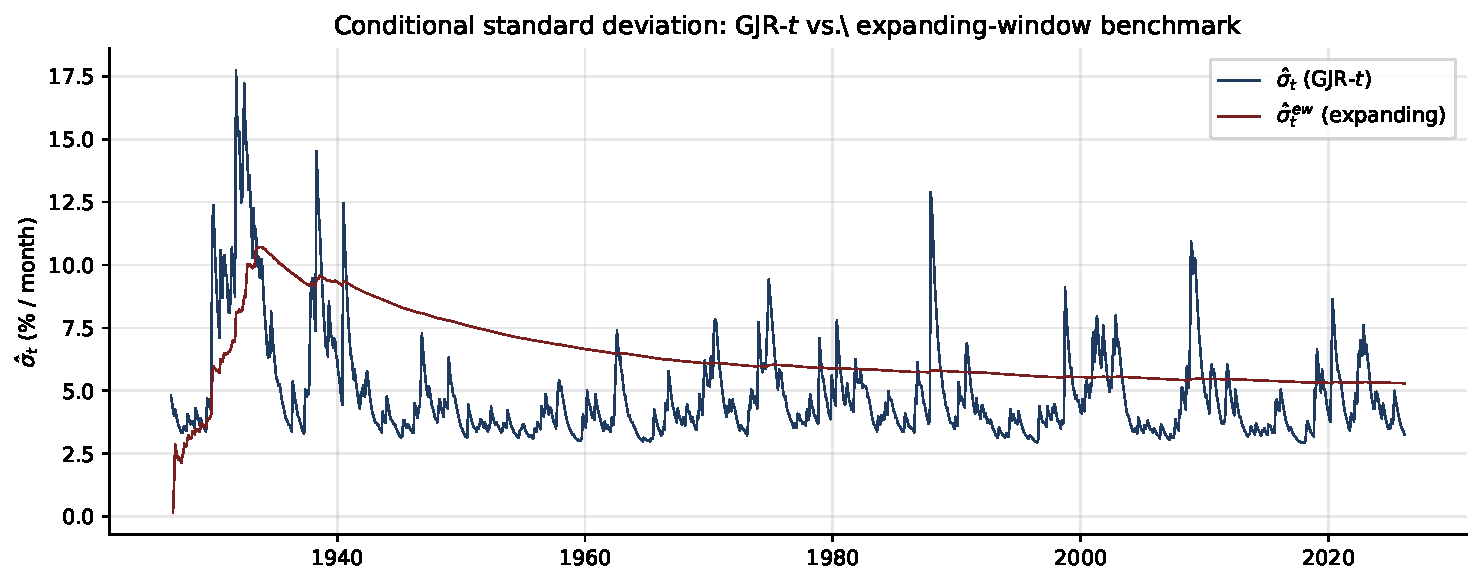
\includegraphics[width=0.92\textwidth]{figures/fig3_sigma.pdf}\\[-2pt]
\caption{Conditional standard deviation: GJR-$t$ vs.\ expanding-window benchmark.}\label{fig:sigma}
\end{figure}\vspace{-0.4em}

\begin{figure}[H]\centering
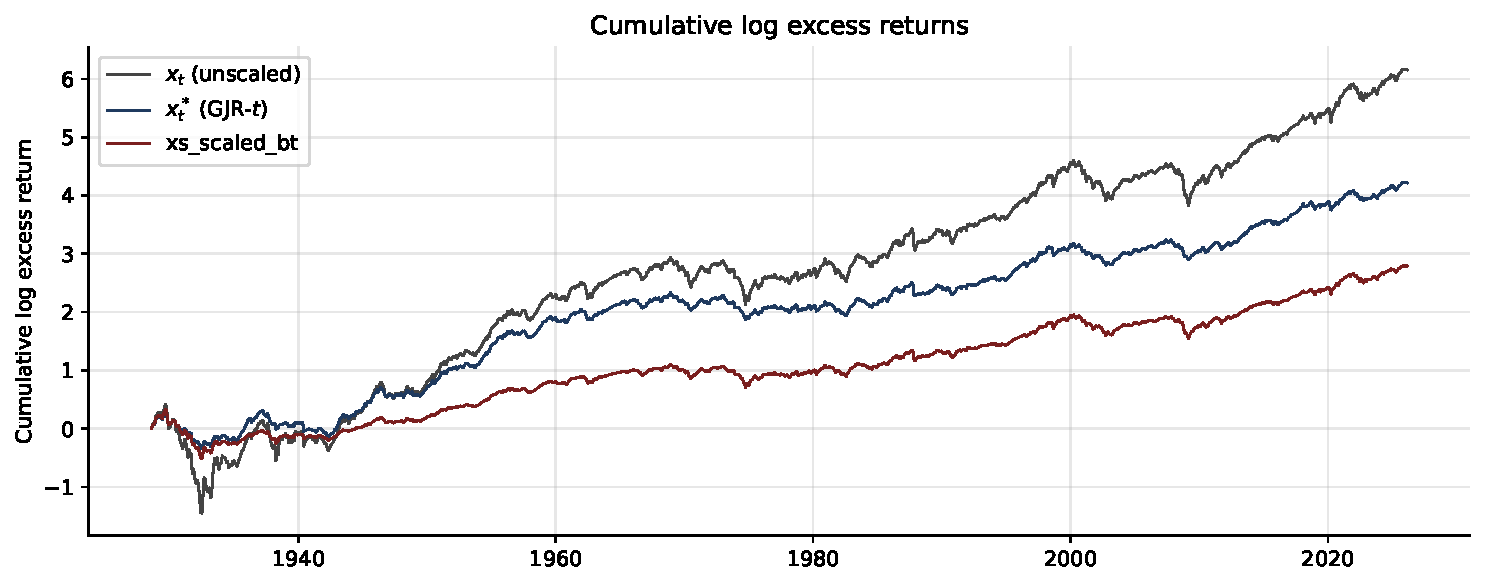
\includegraphics[width=0.92\textwidth]{figures/fig4_cumret.pdf}\\[-2pt]
\caption{Cumulative log excess returns. The volatility-scaled series $x^*_t$ dominates both the unscaled market and the expanding-window benchmark.}\label{fig:cum}
\end{figure}

\end{document}
